\section{Petri Nets Considering Time}
	
	In the formalism of Ordinary Petri Nets, the time is not considered and this results in 
	indeterminism regarding time. It is not specified when a sensibilized transition will be fired 
	or even if it will be fired. Neither can be said which transition from a group of transitions in
	 conflict will be fired \cite{garcia_izquierdo}.
	
	There are three different interpretations about how the time should be consider. All of them 
	have its focus on reducing the indeterminism regarding time in Petri Nets: 
	\begin{itemize}
	  	\renewcommand{\theenumi}{\Alph{enumi}}
	  	\item \underline{Stochastic Petri Net}
			Introduces a stochastic estimation on the instant of firing of a transition.
		\item \underline{Timed Petri Net}
			Introduces a time condition which specifies the duration of the transition.
		\item \underline{Time Petri Net}
			Introduce temporary dimensions between which the transition should be fired.
	\end{itemize}
	
	\begin{figure}[h]
		\centering
		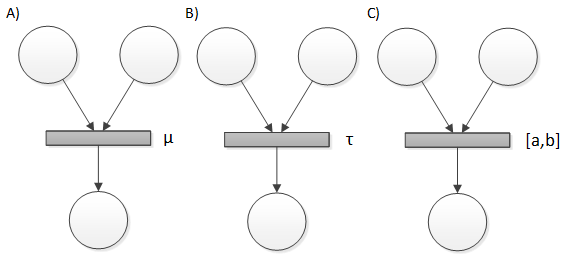
\includegraphics[width=2.8in]{./img/Petri16}
		\caption{Different ways to intruduce time in Petri Nets}
		\label{fig:Petri16}
	\end{figure}
	
	The temporal parameters associated with transitions can be interpreted in these three different ways\footnotemark:
	\footnotetext{ $\bullet t$ is the set of places that are inputs to a
	transition, mathematically defined as: $\bullet t = \{ p \in P : (p , t) \in F \}$.
	
	$t \bullet$ is the set of positions that are outputs of a transition, mathematically defined as: 
		$t \bullet = \{ p \in P : (t , p) \in F \}$.
	
	$F$ is the set of arcs, input and output to the transitions-
	}	
	\begin{enumerate}
		\item Generalized Stochastic Petri Nets (GSPNs) \cite{domeika} have two different types of 
		transitions: immediate transitions and timed transitions. When a transition $t$ is sensitized,
		its firing could be: 
		a) with a duration equal to zero if the transition $t$ is immediate. 
		b) after a lapse of a random time. This random time is expressed by an exponential 
		distribution. The A Net from the figure \ref{fig:Petri16} graphically represents a stochastic timed 
		transition where its probability to be fired is represented by $\mu$.\\
		
		\item Timed Petri Nets have two different types of transitions: immediate transitions and 
		timed transitions. When a transition $t$ is sensitized, its firing could be: 
		a) with a duration equal to zero if the transition $t$ is immediate. 
		b) with immediate removal of tokens from set $\bullet t$ but placing the tokens in the $t\bullet$ 
		only after time $\tau$ has elapsed. Meanwhile, the transition cannot be sensitized. The B Net from the 
		figure \ref{fig:Petri16} graphically represents a timed transition with a delay equal to $\tau$.\\
			
		\item Time Petri Nets have two different types of transitions: immediate transitions and time
		 transitions. When a transition $t$ is sensitized, its firing could be: 
		 a) with a duration equal to zero if the transition $t$ is immediate. 
		 b) if it is a time transition, at the time it is sensitized, a timer starts. The transition 
		 can only be fired when the timer value is between the limits of the interval [a, b]. 
		 Otherwise, the transition cannot be fired. Once the firing was performed, the timer is 
		 restarted. The C Net from the figure \ref{fig:Petri16} graphically represents a time 
		 transition with an associated interval equal to [a, b].\\
	\end{enumerate}
	
	Should be noted that all the firings are performed in two steps: 
	a) the removal of the tokens from the set $\bullet t$. This is an atomic action and the amount 
	of tokens removed from each place is equal to the weight of the arcs joining each place in 
	$\bullet t$ with the transition $t$. b) The atomic action of placing in each place of set $t \bullet$  
	the amount of tokens indicated by the weight of the arcs joining each place of $t \bullet$ with 
	the transition $t$.